\subsubsection{Description}
%Describe your concept of the discharge circuitry.

Discharge circuit's purpose is to discharge capacities connected to \gls{ts} voltage and ensure \gls{ts} safety in shutdown state. Such capacities are only in two \glspl{mc}.
Discharge is activated whenever \gls{sdc} is open. (That means, \gls{acp} is disconnected from \gls{ts} by\glspl{air} ) This behavior is controlled by \gls{ecub}, which monitors latching of \gls{sdc}. It's state is distributed through CAN to other units.
When \gls{sdc} opens, \gls{ecub} sends message to \glspl{mc}, which then closes relays and connects discharge resistors to capacitor bank charged on \gls{ts} voltage.
When \glspl{air} are closed, \gls{ecub} sends message to \gls{mc} to open discharge circuit.

\subsubsection{Wiring, cables, current calculations, connectors}
%\iffalse Describe wiring, show schematics, describe connectors and cables used and show useful data regarding the wiring.
%\begin{itemize}
	%	\item 	Give a plot “Voltage” vs. time 
	%	\item 	Give the formula describing this behavior
	%	\item 	Give a plot “Discharge current” vs. time
	%	\item 	Give the formula describing your plot
%\end{itemize}\fi

\begin{figure}[H]
	\centering
	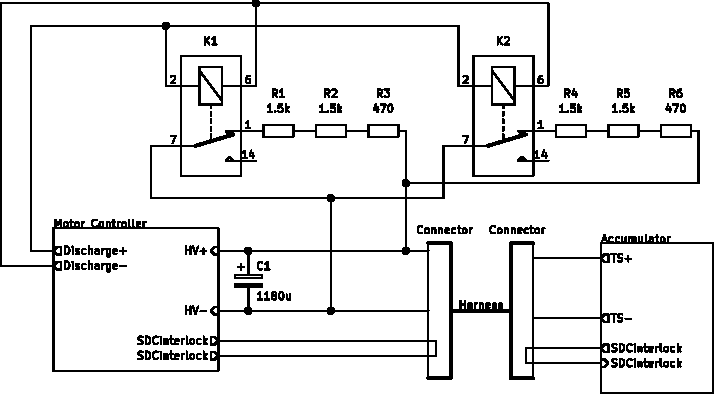
\includegraphics[width=0.7\textwidth]{./img/MC_discharge.pdf}
	\caption{Discharge circuit of one \gls{mc}.}
	\label{fig:discharge-circuit}
\end{figure}

\ref{fig:discharge-circuit} shows a simplified discharge circuitry. Discharge resistors are placed in \glspl{mc} right next to the only capacity that provides a storage for potentially dangerous charge/energy in \gls{ts}. If \gls{hv} cable is disconnected on either side, the \gls{sdc} opens due to the interlocks and both \glspl{air} open. Because there is no output capacitance in \gls{acp} there is no way the power could be on \gls{acp} output \gls{hv} connector.

Capacity sum of all capacitors in \glspl{mc} is 2360 uF. For discharging this capacity in less than 5 seconds to voltage (below 60V), maximum resistor value is calculated by solving R from \ref{eq:discharge_voltage_eq}.

\begin{equation}
	V_{c}=V_{s}*e^{(\frac{-t}{R*C})}
	\label{eq:discharge_voltage_eq}
\end{equation}

\paragraph{Values}
\begin{itemize}
	\item $V_c = 60 V$ (safe voltage limit)
	\item $V_s = 400 V$ (TS voltage)
	\item $t = 5 s$ (maximum discharge time)
	\item $C = 2360\mu$F (total capacity in TS)
\end{itemize}

Maximum resistance from equation \ref{eq:discharge_voltage_eq}, $R = 1112\Omega$ is for discharging all capacitors in \gls{ts}. In our case, capacity is split between two \glspl{mc}. Two parallel resistor combinations of three $1k\Omega$ resistors in series (3s2p) in each \gls{mc} is used (3s4p in total). $1k\Omega$ resistors are PWR221T-30-1001F. Total value of Discharge resistor bank is $R = 750\Omega$, which is less than maximal calculated $R = 1112\Omega$. The 60V threshold with such configuration is reached in $3.37s$. \ref{fig:discharge_voltage_time} shows TS voltage in time during discharging.

\begin{figure}
	\begin{tikzpicture}
		\begin{axis}[
			use units,
			x unit=s,
			y unit=V,
			xlabel=time,
			ylabel=voltage,
			width=0.9\textwidth,
			height=0.5\textwidth,
			grid=major,
			xmin=0,
			ymin=0,
			xmax=20,
			ymax=410
			]
			\addplot[red, smooth] table[
				x=time,
				y=voltage,
				col sep=comma
				] {./data/TS_discharge.csv}; 
			\addplot [mark=none, black, dashed] coordinates {(0, 60) (20, 60)};
			\addplot [mark=none, black, dashed] coordinates {(5, 0) (5, 410)};
		\end{axis}
	\end{tikzpicture}
	\caption{\gls{ts} voltage during discharge. (\glspl{air} open)}
	\label{fig:discharge_voltage_time}
\end{figure}


\begin{figure}
	\begin{tikzpicture}
		\begin{axis}[
			use units,
			x unit=s,
			y unit=A,
			xlabel=time,
			ylabel=current,
			width=0.9\textwidth,
			height=0.5\textwidth,
			grid=major,
			xmin=0,
			ymin=0,
			xmax=20
			]
			\addplot[red, smooth] table[
			x=time,
			y=current,
			col sep=comma
			] {./data/TS_discharge.csv}; 
		\end{axis}
	\end{tikzpicture}
	\caption{Discharge current through resistor bank vs. time}
	\label{fig:discharge_current_time}
\end{figure}



The formula describing \ref{fig:discharge_current_time} is:

\begin{equation}
	I_{d}=\frac{V_{C}-V_{s}}{R_{d}}	
\end{equation}


Where $V_{s}$ is voltage on \gls{ts}, $R_{d}$ is total value of discharge resistor bank and $I_{d}$ is discharge current. Current through individual 3s resistor combinations can be calculated as $I_{d}$/$4$.


\begin{figure}
	\begin{tikzpicture}
		\begin{axis}[
			use units,
			x unit=s,
			y unit=W,
			xlabel=time,
			ylabel=power loss,
			width=0.9\textwidth,
			height=0.5\textwidth,
			grid=major,
			xmin=0,
			ymin=0,
			xmax=20
			]
			%\pgfplotstableread{./data/TS_discharge_current.csv}\dischargeData;
			\addplot[red, smooth] table[
				x=time,
				y expr=(\thisrow{current}/4)^2*3000,
				col sep=comma
				] {./data/TS_discharge.csv}; 
			\addlegendentry{3s resistor combination $P_{loss}$}
			\addplot[orange, smooth] table[
				x=time,
				y expr=(\thisrow{current}/4)^2*1000,
				col sep=comma
				] {./data/TS_discharge.csv};
			\addlegendentry{1 resistor $P_{loss}$}
		\end{axis}
	\end{tikzpicture}
	\caption{Discharge power loss on 3s resistor combination and individual resistors vs. time}
	\label{fig:discharge_power_time}
\end{figure}

Peak power on individual resistors is 18W and resistor can handle up to 30W, see \ref{app:discharge_resistor_sheet}.

\begin{table}[H]
	\centering
	\caption{General data of the discharge circuit}
	\begin{tabularx}{\textwidth}{|X|X|}
		\hline
		Resistor Type: & PWR221T-30-1001F in 3s4p configuration \\[\TableSize]
		\hline
		Resistance: & $1 k\Omega$ \\[\TableSize]
		\hline
		Continuous power rating: & 30 W \\[\TableSize]
		\hline
		Overload power rating (1 sec): & not specified \\[\TableSize]
		\hline
		Overload power rating (5 sec): & not specified \\[\TableSize]
		\hline
		Overload power rating (15 sec): & not specified \\[\TableSize]
		\hline
		Voltage rating: & 250V (3 in series: 750 V) \\[\TableSize]
		\hline
		Maximum expected current: & 0.1 A per resistor, (3s4p configuration with total 0.4A current) \\[\TableSize]
		\hline
		Average current: & 0.04 A through resistor(average from 4 seconds of discharging) \\[\TableSize]
		\hline
		Cross-sectional area of the wire used: & $0.129 mm^2$ \\[\TableSize]
		\hline
	\end{tabularx}%
	\label{tab:dischrage-circ}%
\end{table}%

\begin{table}[H]
	\centering
	\caption{General data of the dis-charge relay}
	\begin{tabularx}{\textwidth}{|X|X|}
		\hline
		Relay Type: & TE PE014012 \\[\TableSize]
		\hline
		Contact arrangement: & 1 pole, normally closed  \\[\TableSize]
		\hline
		Continuous DC current: & 5 A \\[\TableSize]
		\hline
		Voltage rating  & $250 V_{ac}$/$30 V_{dc}$ \footnotemark \\[\TableSize]
		\hline
		Nominal Coil Voltage: 12 V & \\[\TableSize]
		\hline
		Cross-sectional area of the wire used: & $0.129 mm^2$ \\[\TableSize]
		\hline
	\end{tabularx}%
	\label{tab:discharge-relay}%
\end{table}%

\todo[inline]{prilozit datasheet kvuli grafu max proudu a napeti}
\todo[inline]{zminit, ze jedno rele odpojuje jen jednu 3s kombinaci -> 130mA}

\footnotetext{contact is opened when discharge voltage reaches 0V and thus no arcing occurs}


\subsubsection{Position in car}
%Provide CAD-renderings showing all relevant parts. Mark the parts in the rendering, if necessary.

Discharge resistors are mounted on aluminum cooler also with IGBT modules in \gls{mc} boxes.